% Build: pdflatex barn_effect.tex (run twice for references)
\documentclass[11pt]{article}

\usepackage{amsmath,amssymb,amsthm,mathtools}
\usepackage{bm}
\usepackage[margin=1in]{geometry}
\usepackage{hyperref}
\usepackage{tikz}
\usetikzlibrary{decorations.pathreplacing}
\hypersetup{colorlinks=true,linkcolor=blue,citecolor=blue,urlcolor=blue}

\newtheorem{definition}{Definition}
\newtheorem{remark}{Remark}
\newtheorem{proposition}{Proposition}
\newtheorem{assumption}{Assumption}

\title{The Barn Effect: A Streaming Algorithm for\\
Pairwise Feature Attribution on Tabular Data\\
\large Streaming Estimation of Pairwise Conditional Means via an Activation-Parameterized Interaction Graph}
\author{Niklaus Parcell\\
\textit{Mont Ops Inc.\ / Independent Research}\\
\texttt{nik@mont-ops.com}}
\date{May 2026}

\begin{document}
\maketitle

\begin{abstract}
We present \emph{The Barn Effect}, a two-phase algorithm for per-sample feature attribution on tabular data supporting regression, binary classification, and multi-class classification targets.
Conceptually $\bm{\Phi}^\phi$ is a \emph{streaming sufficient-statistic summary} of pairwise stratum-wise outcome structure under a chosen quantization $\mathcal{B}$ and a KG-pair activation $\phi$.
The first phase discretizes each column into a finite set of labeled bins via frequency-ranked boundaries, building a compact vocabulary of value labels shared across all columns.
The second phase accumulates, for every pair of columns and every co-occurring pair of bin labels, an \emph{activation-parameterized conditional mean} of the outcome variable, producing a sparse interaction graph $\bm{\Phi}^\phi$ as the learned model artifact; the reference crate exposes $\phi_{\log}$ (log-frequency damped, default) and $\phi_{\mathrm{mean}}$ (pure conditional mean) as the two standard choices.
Both phases are streaming-compatible, operating on fixed-size chunks without materializing the full dataset.
The outcome $Y^{(n)}$ is \emph{parametric-optional}: it may be the raw target label or the predicted output of any trained model (gradient-boosted trees, random forests, neural networks, etc.), making the algorithm applicable both as a direct data analysis tool and as a model-agnostic explainer.
At inference, each sample's bin labels are routed through $\bm{\Phi}^\phi$ via edge lookups, producing a per-column attribution score $\delta_c^{(n)}$ via effect activation $e$, with default $e_{\mathrm{contrast}}(A, \bar{Y}) = A - \bar{Y}$.
Averaging these scores across rows yields a global feature importance ranking; reading them per-row yields individual prediction explanation.
We provide formal definitions, the activation class and its instances, a strong-law convergence result connecting $\bm{\Phi}^\phi$ to conditional expectation, and complexity bounds scaling as $O(p^2 N)$ in training and $O(p^2)$ per inference sample.
This note develops the definitions and convergence theory for the resulting interaction graph; empirical benchmarks against SHAP, LIME, and ICE are deferred to future work.
\end{abstract}

\section{Introduction}

A recurring challenge in applied machine learning is understanding \emph{which features drive an outcome for a specific sample}, rather than on average across a population.
Global feature importance methods---permutation importance, coefficient magnitudes, tree-based impurity scores---assign a single weight to each feature regardless of what the input values actually are.
Per-sample attribution methods address this gap but often require a differentiable model \cite{Lundberg2017}, a fitted ensemble \cite{Breiman2001}, or a Shapley-value computation whose cost is exponential in the number of features \cite{Ribeiro2016}.

The Barn Effect proceeds differently: it operates directly on the data by recording, for every pair of feature values that co-occur in a training row, what outcome that co-occurrence is associated with.
These pairwise statistics accumulate into a sparse weighted graph $\bm{\Phi}$---the \emph{interaction graph}---whose entries are log-frequency-weighted conditional means of the outcome variable.
At inference, a sample's bin labels are looked up in $\bm{\Phi}$, and the resulting edge weights are aggregated per column to produce attribution scores.

\paragraph{Two-phase structure.}
\begin{enumerate}
  \item \textbf{Training (graph construction).}
    Discretize columns into bins; accumulate co-occurrence statistics over the data in chunks; compute $\bm{\Phi}$ as the completed interaction graph.
  \item \textbf{Inference (edge lookup).}
    Map each row's values to their bin labels; look up the edge weight in $G_\Phi$ for every column pair; aggregate per column to produce the attribution matrix $\bm{\Delta}$.
\end{enumerate}
The model artifact is $\bm{\Phi}$: a sparse matrix of shape $V \times V$, where $V$ is the size of the bin-label vocabulary.
Once trained, $\bm{\Phi}$ can be applied to any number of rows without retraining.

\paragraph{Parametric-optional outcome.}
The outcome $Y^{(n)}$ fed into the accumulator is not required to be the raw data label.
It may equally be the scalar output of any trained model $\hat{f}(\bm{x}^{(n)})$---a gradient-boosted score \cite{Chen2016}, a random forest prediction \cite{Breiman2001}, a neural network logit, or a calibrated probability.
When raw labels are used, the Barn Effect describes the data directly.
When model outputs are used, it explains the model's behavior: which feature co-occurrences are associated with high or low predicted scores.

\paragraph{Streaming scalability.}
A key practical advantage over existing attribution methods is that the Barn Effect never requires the full dataset to be held in memory simultaneously.
SHAP \cite{Lundberg2017} requires a background dataset at inference time, and exact Shapley computation is exponential in $p$; LIME \cite{Ribeiro2016} requires repeated model queries per sample, with neither method natively supporting data streams or datasets that exceed available memory.
The Barn Effect's sufficient statistics $(\bm{W}, \bm{C})$ grow only with the number of distinct co-occurring bin-label pairs---bounded by $O(p^2 B^2)$ regardless of $N$---enabling attribution over arbitrarily large or continuously arriving data without retaining the original dataset \cite{Gama2014,Bifet2018}.
Combined with additive accumulation (Section~\ref{sec:accumulate}), this makes the algorithm applicable to continual and stream-learning settings \cite{Gama2014} where static explainability methods cannot be applied incrementally.

\subsection*{Scope}
We do not claim experimental benchmarks or comparison against existing attribution methods.
We provide definitions, constructions sufficient for implementation, and the mathematical properties of the interaction graph and its derived attribution scores.

\section{Preliminaries and notation}
\label{sec:prelim}

Let $[n] \coloneqq \{1,\ldots,n\}$.
Scalars are Roman or Greek; vectors are bold lower case (e.g., $\bm{v}$); matrices are bold upper case (e.g., $\bm{A}$).
Element-wise matrix operations are written with $\odot$ (product) and $\oslash$ (division on the nonzero support).
For a finite set $S$, $|S|$ denotes its cardinality.

\paragraph{Dataset.}
Let $\mathcal{D} = \{(\bm{x}^{(n)}, Y^{(n)})\}_{n=1}^{N}$ be a tabular dataset with $p$ features and scalar outcome $Y^{(n)} \in \mathbb{R}$.
We write $X_i^{(n)}$ for the value of feature $i \in [p]$ at sample $n$.

\begin{definition}[Outcome]
\label{def:outcome}
$Y^{(n)} \in \mathbb{R}$ is a scalar outcome; see \S\ref{sec:implementation} for parametric-optional usage.
\end{definition}

\paragraph{Column pair set.}
We require $p \ge 2$.
\[
  \mathcal{C} \;\coloneqq\; \bigl\{(i,j) : 1 \le i < j \le p\bigr\}, \qquad |\mathcal{C}| = \tfrac{p(p-1)}{2}.
\]
Data may arrive in $K$ contiguous chunks $\mathcal{D}_1,\ldots,\mathcal{D}_K$ of sizes $n_1,\ldots,n_K$ with $\sum_k n_k = N$.

\section{Phase 1: Discretization}
\label{sec:discretize}

Raw feature values are mapped to discrete bin labels before accumulation.
Discretization limits the vocabulary of value pairs that must be tracked and groups continuous or sparse numerical values into meaningful ranges.

\begin{definition}[Bin schema]
\label{def:bin-schema}
Fix a per-column bin count $B_i \in \mathbb{N}$ for $i \in [p]$, denoting the desired number of output bins.
\begin{itemize}
  \item \textbf{Numerical column $i$.}
    Let $r_i \coloneqq \max_n X_i^{(n)} - \min_n X_i^{(n)}$ be the observed range of column $i$.
    Round all observed values to $s_i$ \emph{decimal places}, where $s_i$ is given by \eqref{eq:si-rounding}.
    Select the top-$B_i$ most frequently occurring rounded values as boundary candidates; sort them and replace the largest with the observed column maximum $b_{B_i}^{(i)} \coloneqq \max_n X_i^{(n)}$; prepend the observed minimum as $b_0^{(i)} \coloneqq \min_n X_i^{(n)}$.
    This yields $B_i + 1$ boundary values $b_0^{(i)} < b_1^{(i)} < \cdots < b_{B_i}^{(i)}$, with $b_1^{(i)},\ldots,b_{B_i-1}^{(i)}$ as the $B_i - 1$ interior split points and the endpoints anchored at the observed data range.
    The bin label assigned to value $x$ is the interval string $[b_k^{(i)},\, b_{k+1}^{(i)})$, where
    $k = \max\bigl\{k' \in \{0,\ldots,B_i-1\} : b_{k'}^{(i)} \le x\bigr\}$.
    This yields exactly $B_i$ non-empty bins.
  \item \textbf{Categorical column $i$.}
    Let $\mathcal{F}_i$ be the $B_i$ most frequently occurring distinct values.
    Any value outside $\mathcal{F}_i$ maps to the distinguished token $\varepsilon$.
    The label set is $\mathcal{L}_i = \mathcal{F}_i \cup \{\varepsilon\}$.
\end{itemize}
The \emph{bin schema} $\mathcal{B} = \{(\mathcal{L}_i,\, \ell^{(i)})\}_{i=1}^{p}$ collects the label sets and the maps $\ell^{(i)} : \mathrm{dom}(X_i) \to \mathcal{L}_i$.
\end{definition}

For numerical columns, the integer $s_i$ adjusts rounding coarseness from the observed range:
\begin{equation}
\label{eq:si-rounding}
  s_i \;\coloneqq\; \max\!\bigl(0,\; 4 - \lfloor \log_{10}(r_i) \rfloor\bigr),
\end{equation}
so wider $r_i$ yields coarser rounding and narrower $r_i$ finer rounding (e.g., $r_i \approx 1$ gives $s_i = 4$; $r_i \approx 1000$ gives $s_i = 1$).

\paragraph{Missing inputs before binning.}
The maps $\ell^{(i)}$ are applied only after a practitioner-chosen \emph{missing-input convention} maps raw cells to inputs in $\mathrm{dom}(X_i)$.
One default convention replaces numerical \texttt{NaN} with zero before bin assignment, treats categorical \texttt{NaN} as \texttt{empty} (mapping to $\varepsilon$ when infrequent), and replaces outcome \texttt{NaN} with zero so such rows contribute zero to $W_{uv}$.
Histograms used for frequencies, endpoints $\min/\max$, and hence $r_i$ and $\mathcal{B}_N$, are computed from these \emph{effective} values, so systematic missingness can concentrate mass on imputed atoms and couples $\mathcal{B}_N$ to the missing-data rule (potentially analogous to MAR/MNAR issues in exploratory analysis).

Figure~\ref{fig:num-bins} illustrates numerical binning with $B=4$: the top-4 most frequent values are selected as boundary candidates; the largest is replaced by the column maximum, leaving three interior split points and yielding exactly $B=4$ bins.
Figure~\ref{fig:cat-bins} illustrates categorical selection with $B=4$: the four most frequent categories are retained; all others collapse to $\varepsilon$.

\begin{figure}[ht]
\centering
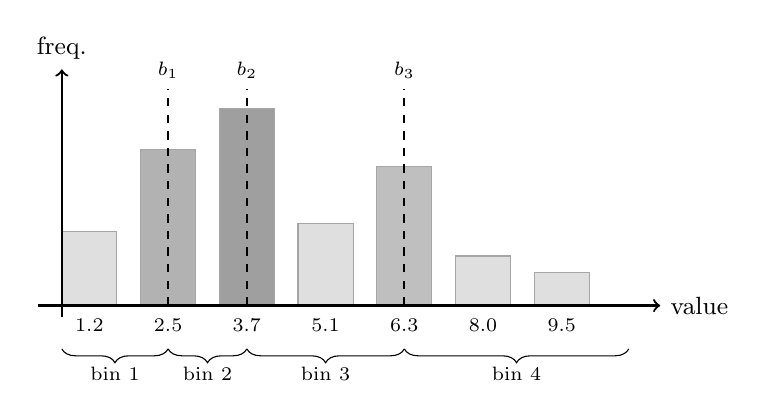
\begin{tikzpicture}[scale=1.0]
  % 7 bars, bar width 0.7, pitch 1.0
  % Freqs: 45,95,120,50,85,30,20. Heights scaled to max=2.5 (scale=2.5/120)
  % Top-3 by freq: idx2(120), idx1(95), idx4(85) -> boundary bars darker
  % Sorted boundaries: b1=val at idx1=2.5, b2=val at idx2=3.7, b3=val at idx4=6.3
  % Bar centers: 0.35,1.35,2.35,3.35,4.35,5.35,6.35

  % Non-boundary bars
  \fill[gray!25] (0.0,0) rectangle (0.70,0.94);
  \fill[gray!25] (3.0,0) rectangle (3.70,1.04);
  \fill[gray!25] (5.0,0) rectangle (5.70,0.63);
  \fill[gray!25] (6.0,0) rectangle (6.70,0.42);
  % Boundary bars (darker)
  \fill[gray!60] (1.0,0) rectangle (1.70,1.98);
  \fill[gray!75] (2.0,0) rectangle (2.70,2.50);
  \fill[gray!50] (4.0,0) rectangle (4.70,1.77);
  % Outlines
  \foreach \xa/\xb/\h in {%
    0.0/0.70/0.94, 1.0/1.70/1.98, 2.0/2.70/2.50,
    3.0/3.70/1.04, 4.0/4.70/1.77, 5.0/5.70/0.63, 6.0/6.70/0.42} {
    \draw[gray!70] (\xa,0) rectangle (\xb,\h);
  }
  % Axes
  \draw[->,thick] (-0.3,0) -- (7.6,0) node[right,font=\small] {value};
  \draw[->,thick] (0,-0.15) -- (0,3.0) node[above,font=\small] {freq.};
  % X-axis value labels
  \foreach \xc/\v in {0.35/1.2, 1.35/2.5, 2.35/3.7, 3.35/5.1, 4.35/6.3, 5.35/8.0, 6.35/9.5} {
    \node[below,font=\scriptsize] at (\xc,-0.05) {\v};
  }
  % Dashed boundary lines at bar centers of top-4 candidates (start at axis)
  \draw[dashed,thick] (1.35,0) -- (1.35,2.75)
    node[above,font=\scriptsize] {$b_1$};
  \draw[dashed,thick] (2.35,0) -- (2.35,2.75)
    node[above,font=\scriptsize] {$b_2$};
  \draw[dashed,thick] (4.35,0) -- (4.35,2.75)
    node[above,font=\scriptsize] {$b_3$};
  % Underbrace bin labels (B=4 bins)
  \draw[decorate,decoration={brace,amplitude=5pt,mirror}]
    (0.00,-0.55) -- (1.35,-0.55)
    node[midway,below,yshift=-3pt,font=\scriptsize] {bin 1};
  \draw[decorate,decoration={brace,amplitude=5pt,mirror}]
    (1.35,-0.55) -- (2.35,-0.55)
    node[midway,below,yshift=-3pt,font=\scriptsize] {bin 2};
  \draw[decorate,decoration={brace,amplitude=5pt,mirror}]
    (2.35,-0.55) -- (4.35,-0.55)
    node[midway,below,yshift=-3pt,font=\scriptsize] {bin 3};
  \draw[decorate,decoration={brace,amplitude=5pt,mirror}]
    (4.35,-0.55) -- (7.20,-0.55)
    node[midway,below,yshift=-3pt,font=\scriptsize] {bin 4};
\end{tikzpicture}
\caption{Numerical bin schema with $B=4$ bins.
  The top-4 most frequent rounded values are the boundary candidates (darker bars); the largest is replaced by the observed column maximum, leaving three interior split points $b_1,b_2,b_3$ (dashed lines) and yielding $B=4$ bins.}
\label{fig:num-bins}
\end{figure}

\begin{figure}[ht]
\centering
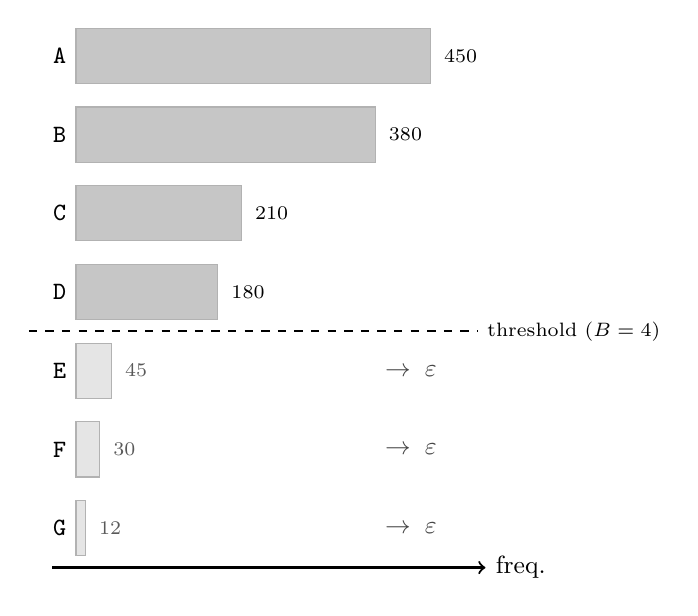
\begin{tikzpicture}[scale=1.0]
  % 7 horizontal bars, y positions: A@6,B@5,C@4,D@3,E@2,F@1,G@0
  % Bar height 0.7, from y+0.15 to y+0.85
  % Widths scaled: 450->4.50, 380->3.80, 210->2.10, 180->1.80, 45->0.45, 30->0.30, 12->0.12
  % B=4 kept: A,B,C,D; below threshold: E,F,G
  % Threshold line at y=2.5 (midpoint between D bottom=3.15 and E top=2.85 -- wait)
  % D bar: y=3.15 to 3.85; E bar: y=2.15 to 2.85 -> threshold at y=3.0

  % Kept bars
  \fill[gray!45] (0,6.15) rectangle (4.50,6.85);
  \fill[gray!45] (0,5.15) rectangle (3.80,5.85);
  \fill[gray!45] (0,4.15) rectangle (2.10,4.85);
  \fill[gray!45] (0,3.15) rectangle (1.80,3.85);
  % Below-threshold bars
  \fill[gray!20] (0,2.15) rectangle (0.45,2.85);
  \fill[gray!20] (0,1.15) rectangle (0.30,1.85);
  \fill[gray!20] (0,0.15) rectangle (0.12,0.85);
  % Outlines
  \foreach \ya/\yb/\w in {%
    6.15/6.85/4.50, 5.15/5.85/3.80, 4.15/4.85/2.10, 3.15/3.85/1.80,
    2.15/2.85/0.45, 1.15/1.85/0.30, 0.15/0.85/0.12} {
    \draw[gray!60] (0,\ya) rectangle (\w,\yb);
  }
  % Category labels on the left
  \foreach \y/\lab in {6.50/A, 5.50/B, 4.50/C, 3.50/D, 2.50/E, 1.50/F, 0.50/G} {
    \node[left,font=\small] at (0,\y) {\texttt{\lab}};
  }
  % Frequency values after bars
  \foreach \y/\w/\f in {6.50/4.50/450, 5.50/3.80/380, 4.50/2.10/210, 3.50/1.80/180} {
    \node[right,font=\scriptsize] at (\w+0.05,\y) {\f};
  }
  \foreach \y/\w/\f in {2.50/0.45/45, 1.50/0.30/30, 0.50/0.12/12} {
    \node[right,font=\scriptsize,gray!70!black] at (\w+0.05,\y) {\f};
  }
  % -> epsilon for below-threshold
  \foreach \y in {2.50, 1.50, 0.50} {
    \node[right,font=\small,gray!55!black] at (3.8,\y) {$\to\;\varepsilon$};
  }
  % Dashed threshold line between D (bottom=3.15) and E (top=2.85), at y=3.0
  \draw[dashed,thick] (-0.6,3.0) -- (5.1,3.0);
  \node[right,font=\scriptsize] at (5.1,3.0) {threshold ($B=4$)};
  % x-axis
  \draw[->,thick] (-0.3,0) -- (5.2,0) node[right,font=\small] {freq.};
\end{tikzpicture}
\caption{Categorical bin schema with $B=4$.
  The four most frequent categories (\texttt{A}--\texttt{D}) are retained; the remaining three fall below the frequency threshold and are mapped to the distinguished token $\varepsilon$.}
\label{fig:cat-bins}
\end{figure}

\begin{definition}[Bin-label vocabulary]
\label{def:vocab}
Let $\mathcal{V} \coloneqq \bigcup_{i=1}^{p} \mathcal{L}_i$ be the set of all bin labels produced by $\mathcal{B}$, with $V \coloneqq |\mathcal{V}|$.
Identify $\mathcal{V}$ with $[V]$ via a fixed ordering established during discretization.
From this point forward, bin labels are integers in $[V]$; in particular, $\ell^{(i)}(X_i^{(n)}) \in [V]$ for all $i$ and $n$.
\end{definition}

\begin{remark}[Column-specific labels]
\label{rem:col-specific}
Each label set $\mathcal{L}_i$ is disjoint from $\mathcal{L}_j$ for $i \neq j$: the encoding assigns distinct integers to labels from different columns even when their raw values are identical.
As a result, any $u \in \mathcal{L}_i$ and $v \in \mathcal{L}_j$ with $i \neq j$ are always distinct integers in $[V]$, and the diagonal $\Phi_{u,u}$ is never populated by cross-column pairs.
\end{remark}

\begin{remark}[Streaming compatibility of Phase~1]
\label{rem:stream-phase1}
The bin schema $\mathcal{B}$ can be finalized in a single forward pass without reloading any chunk: accumulate per-column rounded-value counts, min, and max across chunks; rank frequencies and assign boundaries once after the final chunk.
\end{remark}

\section{Phase 2: Pairwise accumulation and graph construction}
\label{sec:accumulate}
\label{sec:graph}

After discretization, all feature values are integers in $[V]$.
Phase~2 processes every column pair, accumulates sufficient statistics for each co-occurring value pair, and finalizes the interaction graph $\bm{\Phi}$.

\begin{definition}[Value pair]
\label{def:value-pair}
For sample $n$ and column pair $(i,j) \in \mathcal{C}$, the \emph{value pair} is
\[
  (u,v) \;\coloneqq\; \bigl(\ell^{(i)}(X_i^{(n)}),\; \ell^{(j)}(X_j^{(n)})\bigr) \;\in\; [V]^2.
\]
\end{definition}

\begin{definition}[Canonical value-pair key]
\label{def:canonical-key}
For encoded labels $u,v \in [V]$, define the \emph{canonical key}
\[
  \kappa(u,v) \;\coloneqq\; \bigl(\min\{u,v\},\,\max\{u,v\}\bigr).
\]
All accumulation and lookup use $\kappa\bigl(\ell^{(i)}(X_i^{(n)}),\,\ell^{(j)}(X_j^{(n)})\bigr)$.
\end{definition}

\begin{definition}[Streaming accumulator]
\label{def:accumulator}
Maintain two sparse matrices $\bm{W}, \bm{C} \in \mathbb{R}^{V \times V}$, initialized to $\bm{0}$.
Fix a significance rate $\alpha \in [0,1)$ (default $\alpha = 0.01$).
For chunk $\mathcal{D}_k$ with $n_k \coloneqq |\mathcal{D}_k|$, set $\theta_k \coloneqq \lfloor \alpha n_k \rfloor$.
For each column pair $(i,j) \in \mathcal{C}$ and canonical key $\kappa = \kappa(u,v)$ realized in $\mathcal{D}_k$, let
\[
  c_{\kappa}^{(k)} \;\coloneqq\;
  \bigl|\bigl\{n \in \mathcal{D}_k :
  \kappa\bigl(\ell^{(i)}(X_i^{(n)}),\,\ell^{(j)}(X_j^{(n)})\bigr) = \kappa\bigr\}\bigr|.
\]
If $c_{\kappa}^{(k)} > \theta_k$, define the per-chunk increments
\begin{align}
  \Delta W_{\kappa}^{(k)} \;\coloneqq\;
  \sum_{\substack{n \in \mathcal{D}_k :\\ \kappa\bigl(\ell^{(i)}(X_i^{(n)}),\,\ell^{(j)}(X_j^{(n)})\bigr)=\kappa}} Y^{(n)},
  \label{eq:W-update}\\[6pt]
  \Delta C_{\kappa}^{(k)} \;\coloneqq\; c_{\kappa}^{(k)};
  \label{eq:C-update}
\end{align}
otherwise set $\Delta W_{\kappa}^{(k)} = \Delta C_{\kappa}^{(k)} = 0$.
After all $K$ chunks,
\[
  W_{\kappa} \;\coloneqq\; \sum_{k=1}^{K} \Delta W_{\kappa}^{(k)}, \qquad
  C_{\kappa} \;\coloneqq\; \sum_{k=1}^{K} \Delta C_{\kappa}^{(k)},
\]
indexed by the canonical key $\kappa(u,v)$.
\end{definition}

\begin{remark}[Additive accumulation]
\label{rem:incremental}
Passing increments \eqref{eq:W-update}--\eqref{eq:C-update} are additive over disjoint chunks, so new data may be incorporated by resuming from existing $(\bm{W}, \bm{C})$ totals.
When $\theta_k = 0$ for all $k$, $W_{\kappa}$ and $C_{\kappa}$ depend only on $\mathcal{D}$, not on its partition; with $\theta_k > 0$, borderline pairs may depend on chunking.
Consequently, $(\bm{W}, \bm{C})$ are sufficient statistics for $\bm{\Phi}$ given the chosen partition and thresholds.
\end{remark}

\begin{definition}[KG-pair activation]
\label{def:kg-activation}
A \emph{KG-pair activation} is any function $\phi : \mathbb{R} \times \mathbb{R}_{\ge 0} \to \mathbb{R}$ satisfying the boundary convention
\[
  \phi(s, 0) \;=\; \phi(s, 1) \;=\; 0 \qquad \text{for all } s \in \mathbb{R}.
\]
The \emph{activation class of interest} for this paper consists of functions of the form
\begin{equation}
  \phi(s, c) \;=\; \frac{s}{c} \cdot g(c) \qquad (c > 1),
  \label{eq:phi-class}
\end{equation}
where $g : (1, \infty) \to \mathbb{R}_{> 0}$ is continuous. Concrete instances:
\begin{itemize}
  \item $\phi_{\log}(s, c) \coloneqq (s/c) \cdot \log_{10}(c)$, i.e.\ $g = \log_{10}$ --- the \emph{default} used by the reference crate;
  \item $\phi_{\mathrm{mean}}(s, c) \coloneqq s/c$, i.e.\ $g \equiv 1$ --- pure conditional mean, implemented alongside the default;
  \item $\phi_{\log\!1\mathrm{p}}(s, c) \coloneqq (s/c) \cdot \log_{10}(c + 1)$, i.e.\ $g(c) = \log_{10}(c+1)$ --- a singleton-tolerant illustration kept paper-only.
\end{itemize}
The boundary convention $\phi(s, 1) = 0$ is a deliberate suppression of singleton-cell estimates: it agrees with the natural boundary for $\phi_{\log}$ (since $\log_{10}(1) = 0$) and is enforced as a convention for the rest of the class so that the singleton-cell suppression matches across activations.
\end{definition}

\begin{definition}[Interaction graph under $\phi$]
\label{def:graph}
Fix a KG-pair activation $\phi$ (Definition~\ref{def:kg-activation}).
The \emph{interaction graph under $\phi$} is the sparse matrix $\bm{\Phi}^\phi \in \mathbb{R}^{V \times V}$ with entries
\begin{equation}
  \Phi^\phi_{uv} \;\coloneqq\; \phi(W_{uv},\, C_{uv}).
  \label{eq:Phi}
\end{equation}
Restricted to the class~\eqref{eq:phi-class}, this evaluates to
\[
  \Phi^\phi_{uv} \;=\;
  \begin{cases}
    0 & \text{if } C_{uv} \in \{0, 1\}, \\[6pt]
    \dfrac{W_{uv}}{C_{uv}} \cdot g(C_{uv}) & \text{if } C_{uv} > 1.
  \end{cases}
\]
The default choice $\phi = \phi_{\log}$ recovers $\Phi^{\phi_{\log}}_{uv} = (W_{uv}/C_{uv})\cdot\log_{10}(C_{uv})$, equivalently $\bm{\Phi}^{\phi_{\log}} = (\bm{W} \oslash \bm{C}) \odot \log_{10}(\bm{C})$ on $\{(u,v) : C_{uv} > 1\}$. When the activation is the default we write simply $\bm{\Phi}$ and $\Phi_{uv}$.
\end{definition}

The matrix $\bm{\Phi}^\phi$ is the weighted adjacency matrix of the \emph{interaction graph}
\[
  G_\Phi \;=\; \bigl(\mathcal{V},\; E_\Phi,\; w_\Phi\bigr),
\]
where $\mathcal{V} = [V]$ is the bin-label vocabulary, $E_\Phi = \{(u,v) : \Phi^\phi_{uv} \neq 0\}$ is the edge set, and $w_\Phi(u,v) = \Phi^\phi_{uv}$ is the edge weight function.
We use $\bm{\Phi}^\phi$ and $G_\Phi$ interchangeably: $\bm{\Phi}^\phi$ for matrix operations, $G_\Phi$ for graph language.
The boundary cases $C_{uv} \in \{0, 1\}$ both yield $\Phi^\phi_{uv} = 0$ by the convention of Definition~\ref{def:kg-activation}: for $\phi_{\log}$ this is also analytic since $\log_{10}(1) = 0$, while for the rest of the class it is the deliberate singleton-cell suppression.

\begin{remark}[Undirected edges]
\label{rem:symmetry}
The co-occurrence event ``column $i$ at bin $u$, column $j$ at bin $v$'' is identical to ``column $j$ at bin $v$, column $i$ at bin $u$'': there is no inherent direction.
The accumulator stores each event under the canonical key $\kappa(u,v)$ (Definition~\ref{def:canonical-key}); the interaction graph $G_\Phi$ is therefore undirected.
\end{remark}

\section{Inference: attribution from the interaction graph}
\label{sec:attribution}

\begin{definition}[Per-sample pairwise score]
\label{def:pairwise-score}
Fix a KG-pair activation $\phi$ (Definition~\ref{def:kg-activation}).
For sample $n$ and column pair $(i,j) \in \mathcal{C}$, the \emph{pairwise score} is
\begin{equation}
  \psi_{ij}^{(n)} \;\coloneqq\;
  \Phi^\phi_{\,\kappa\bigl(\ell^{(i)}(X_i^{(n)}),\,\ell^{(j)}(X_j^{(n)})\bigr)}.
  \label{eq:psi}
\end{equation}
This is a single entry lookup in $G_\Phi$ under the canonical key $\kappa$.
If the key is absent from $E_\Phi$, then $\psi_{ij}^{(n)} = 0$.
\end{definition}

\begin{definition}[Column attribution score $A_c^{(n)}$]
\label{def:col-attr}
Let $m_c \coloneqq p - 1$ be the number of column partners for feature $c$.
The \emph{column attribution score} is
\begin{equation}
  A_c^{(n)} \;\coloneqq\;
  \frac{1}{m_c} \sum_{\substack{j=1\\j\neq c}}^{p} \psi_{cj}^{(n)}.
  \label{eq:col-attr}
\end{equation}
Absent pairs enter as zero and are averaged with all partners.
\end{definition}

\begin{remark}[Shared pairwise edges]
\label{rem:shared-edges}
Each entry $\Phi_{uv}$ of the interaction graph contributes to the attribution of \emph{both} the column that produced label $u$ and the column that produced label $v$.
The same edge weight appears in $A_c^{(n)}$ for column $c$ and in $A_{c'}^{(n)}$ for any other column $c'$ that shares an encoded bin in that pair.
Unlike Shapley-based methods, the Barn Effect makes no attempt to allocate the joint effect of a co-occurrence to one side: both columns ``see'' the same signal, and the user interprets their attributions as correlated evidence rather than a partition of a fixed budget.
\end{remark}

\begin{definition}[Effect activation]
\label{def:effect-activation}
An \emph{effect activation} is any function $e : \mathbb{R} \times \mathbb{R} \to \mathbb{R}$ combining a column attribution score with a baseline.
The default is the \emph{global-mean contrast}
\[
  e_{\mathrm{contrast}}(A, \bar{Y}) \;\coloneqq\; A - \bar{Y},
\]
which produces the Barn attribution below.
Alternative effect activations (e.g.\ standardized contrasts) are left for future work; the reference crate currently exposes only $e_{\mathrm{contrast}}$.
\end{definition}

\begin{definition}[Barn attribution]
\label{def:delta}
Let $\bar{Y} \coloneqq N^{-1}\sum_{n=1}^{N} Y^{(n)}$ be the global outcome mean.
Given an effect activation $e$ (Definition~\ref{def:effect-activation}), the \emph{Barn attribution} for column $c$ at sample $n$ is
\begin{equation}
  \delta_c^{(n)} \;\coloneqq\; e\bigl(A_c^{(n)},\, \bar{Y}\bigr).
  \label{eq:delta}
\end{equation}
With the default $e = e_{\mathrm{contrast}}$ this reduces to $\delta_c^{(n)} = A_c^{(n)} - \bar{Y}$: a positive value indicates that column $c$'s pairwise context in row $n$ is associated with outcomes above the global mean; a negative value indicates the opposite.
\end{definition}

\begin{remark}[No efficiency axiom]
\label{rem:no-efficiency}
Unlike SHAP, the Barn Effect does not satisfy the \emph{efficiency axiom}: there is no guarantee that
\[
  \sum_{c=1}^{p} \delta_c^{(n)} \;=\; Y^{(n)} - \bar{Y}.
\]
The attributions $\delta_c^{(n)}$ are not a decomposition of the outcome gap into per-feature shares; they are \emph{estimated descriptions} of how strongly each feature's pairwise context is associated with a deviation from the baseline.
Two features may both exhibit positive attributions without their sum equaling the observed deviation, because each $\delta_c^{(n)}$ is computed from an independent average over pairwise interactions, not from an additive partition of a fixed budget.
\end{remark}

The full output of inference is the \emph{attribution matrix} $\bm{\Delta} \in \mathbb{R}^{N \times p}$ with $\Delta_{nc} = \delta_c^{(n)}$.

\begin{definition}[Global feature importance]
\label{def:global}
The \emph{global importance} of feature $c$ is the mean Barn attribution across all samples:
\begin{equation}
  \bar{\delta}_c \;\coloneqq\; \frac{1}{N} \sum_{n=1}^{N} \delta_c^{(n)}.
  \label{eq:global}
\end{equation}
\end{definition}


\section{Properties}
\label{sec:props}

\begin{remark}[Chunk-additive accumulation]
\label{prop:chunk-additive}
Increments \eqref{eq:W-update}--\eqref{eq:C-update} are additive over disjoint chunks for pairs that pass the per-chunk threshold $\theta_k$ in every chunk where they appear.
When $\theta_k = 0$ for all $k$, totals $W_{\kappa}$ and $C_{\kappa}$ agree with a single pass over $\mathcal{D}$; otherwise partition may affect borderline pairs.
\end{remark}

\begin{proposition}[Complexity]
\label{prop:complexity}
Let $N$ be the total sample count, $p$ the feature count, and $B = \max_i B_i$ the maximum bin depth.
\begin{enumerate}
  \item \textbf{Training.} Processing all $K$ chunks requires $O(p^2 N)$ scalar operations.
    Space for $\bm{W}$ and $\bm{C}$ is $O(p^2 B^2)$ entries in the worst case.
  \item \textbf{Inference.} Computing $\bm{\Delta}$ for a batch of $M$ samples requires $O(p^2 M)$ hash-map lookups, each $O(1)$ expected.
\end{enumerate}
\end{proposition}

\begin{proof}[Proof sketch]
$|\mathcal{C}| = p(p-1)/2$.
For each chunk of size $n_k$, processing one column pair requires stacking $n_k$ value pairs and computing unique counts in $O(n_k)$ via vectorized sort or hash; summing over all pairs and chunks gives $O(p^2 N)$.
Each column pair contributes at most $B^2$ distinct encoded pairs, so $|\mathcal{C}| \cdot B^2 = O(p^2 B^2)$ accumulator entries in total.
At inference, $A_c^{(n)}$ requires $p-1$ lookups per column over $p$ columns: $O(p^2)$ per sample.
\end{proof}

\begin{assumption}[Fixed quantization for asymptotics]
\label{asm:fixed-bins}
Throughout Section~\ref{sec:props}, and in particular Proposition~\ref{prop:convergence}, the bin schema $\mathcal{B}$ and the quantization maps $\ell^{(i)}$ are \emph{nonrandom} measurable functions of the covariates fixed \emph{before} taking limits in $N$: the strata $\{\ell^{(i)}(X_i)=u,\,\ell^{(j)}(X_j)=v\}$ and the masses $\pi$ in Proposition~\ref{prop:convergence} are thus well-defined under the data-generating measure and do not vary with sample size.
Section~\ref{sec:discretize} instead prescribes a sample-constructed schema $\mathcal{B}_N$---random and $N$-dependent.
Practitioners configure the depth $B_i$ and the frequency-based construction (see also \S\ref{sec:implementation}); one operational way to approximate Assumption~\ref{asm:fixed-bins} is to freeze $\mathcal{B}$ from a pilot or hold-out slice, then accumulate $\bm{W},\bm{C}$ on fresh data drawn from the same regime.
Extending Proposition~\ref{prop:convergence} to jointly random $(\mathcal{B}_N,\bm{\Phi})$ requires additional analysis; we do not pursue it here.
\end{assumption}

\begin{proposition}[Convergence of $\bm{\Phi}^\phi$ to scaled conditional expectation]
\label{prop:convergence}
Assume Assumption~\ref{asm:fixed-bins}.
Suppose $\{(\bm{x}^{(n)}, Y^{(n)})\}$ are i.i.d.\ with $\mathbb{E}[|Y|] < \infty$.
Fix $(i,j) \in \mathcal{C}$ and $(u,v) \in [V]^2$ with $\pi \coloneqq P(\ell^{(i)}(X_i)=u,\,\ell^{(j)}(X_j)=v) > 0$.
Let $\phi(s, c) = (s/c) \cdot g(c)$ belong to the activation class of Definition~\ref{def:kg-activation}, and assume the \emph{class condition}
\begin{equation}
  \frac{g(c)}{g(N\pi)} \;\xrightarrow{\;\mathrm{a.s.}\;}\; 1
  \qquad \text{along trajectories with } c, N \to \infty \text{ and } c/N \to \pi > 0.
  \label{eq:class-cond}
\end{equation}
Then
\begin{equation}
  \frac{\Phi^\phi_{uv}}{g(N\pi)}
  \;\xrightarrow{\;\mathrm{a.s.}\;}\;
  \mathbb{E}\!\bigl[Y \mid \ell^{(i)}(X_i)=u,\;\ell^{(j)}(X_j)=v\bigr]
  \quad\text{as } N\to\infty.
  \label{eq:convergence}
\end{equation}
Both default activations of interest satisfy~\eqref{eq:class-cond} (Remark~\ref{rem:class-cond}).
\end{proposition}

\begin{proof}
The argument is three labelled SLLN steps combined by Slutsky.

\textbf{Step 1 (count-side SLLN).}
The indicators $E_n \coloneqq \mathbf{1}\{\ell^{(i)}(X_i^{(n)}) = u,\; \ell^{(j)}(X_j^{(n)}) = v\}$ are i.i.d.\ Bernoulli$(\pi)$. By the strong law of large numbers \cite[Thm.~2.4.1]{Durrett2019},
\[
  \frac{C_{uv}}{N} \;=\; \frac{1}{N}\sum_{n=1}^{N} E_n \;\xrightarrow{\mathrm{a.s.}}\; \pi.
\]
In particular $C_{uv} \to \infty$ a.s.\ since $\pi > 0$.

\textbf{Step 2 (stratum sub-sample SLLN).}
Let $\tau(k)$ denote the index of the $k$-th sample with $E_{\tau(k)} = 1$. Because $\{(\bm{x}^{(n)}, Y^{(n)})\}$ are i.i.d., the sub-sequence $\{Y^{(\tau(k))}\}_{k \ge 1}$ is itself i.i.d.\ with common law $\mathcal{L}(Y \mid E_1 = 1)$ and mean
\[
  \mu \;\coloneqq\; \mathbb{E}\!\bigl[Y \mid \ell^{(i)}(X_i) = u,\; \ell^{(j)}(X_j) = v\bigr],
\]
finite since $\mathbb{E}|Y| < \infty$. Applying the SLLN \cite[Thm.~2.4.1]{Durrett2019} to this sub-sequence on the prob-$1$ event $\{C_{uv} \to \infty\}$ from Step~1,
\[
  \frac{W_{uv}}{C_{uv}} \;=\; \frac{1}{C_{uv}}\sum_{k=1}^{C_{uv}} Y^{(\tau(k))}
  \;\xrightarrow{\mathrm{a.s.}}\; \mu.
\]

\textbf{Step 3 (continuous mapping for $g$).}
By Step~1, the realized trajectory $(c, N) = (C_{uv}, N)$ satisfies $c/N \to \pi$ a.s.\ with $c, N\pi \to \infty$ a.s.; the class condition~\eqref{eq:class-cond} then yields
\[
  \frac{g(C_{uv})}{g(N\pi)} \;\xrightarrow{\mathrm{a.s.}}\; 1.
\]

\textbf{Combine (Slutsky).}
For $C_{uv} > 1$, which holds eventually a.s., $\Phi^\phi_{uv} = (W_{uv}/C_{uv}) \cdot g(C_{uv})$, so
\[
  \frac{\Phi^\phi_{uv}}{g(N\pi)}
  \;=\; \frac{W_{uv}}{C_{uv}} \cdot \frac{g(C_{uv})}{g(N\pi)}
  \;\xrightarrow{\mathrm{a.s.}}\; \mu \cdot 1 \;=\; \mu,
\]
which is~\eqref{eq:convergence}.
\end{proof}

\begin{remark}[Verification of the class condition]
\label{rem:class-cond}
For $g \equiv 1$ (giving $\phi_{\mathrm{mean}}$) the class condition~\eqref{eq:class-cond} holds trivially: $g(c)/g(N\pi) = 1$, and Proposition~\ref{prop:convergence} reduces to $W_{uv}/C_{uv} \xrightarrow{\mathrm{a.s.}} \mathbb{E}[Y \mid u,v]$.

For $g = \log_{10}$ (giving the default $\phi_{\log}$), write
\[
  \frac{\log_{10}(c)}{\log_{10}(N\pi)}
  \;=\; 1 \;+\; \frac{\log_{10}\!\bigl(c / (N\pi)\bigr)}{\log_{10}(N\pi)}.
\]
On the trajectory $c/N \to \pi$ from Step~1, $c/(N\pi) \to 1$ a.s.; continuity of $\log_{10}$ at $1$ gives $\log_{10}(c/(N\pi)) \to 0$ a.s., while the denominator $\log_{10}(N\pi) \to \infty$, so the ratio tends to $1$. This is the \emph{only} place a logarithm identity is invoked, and it appears throughout as a bounded ratio rather than as an equality between two divergent quantities.
\end{remark}

\begin{remark}
Proposition~\ref{prop:convergence} shows $\Phi^\phi_{uv}$ is a consistent, $g$-scaled estimator of the conditional mean.
Under $\phi_{\mathrm{mean}}$ the activation directly estimates $\mathbb{E}[Y \mid u,v]$ on the support $C_{uv} > 1$; under the default $\phi_{\log}$, entries for frequently co-occurring pairs (large $C_{uv}$) receive larger absolute weights, damping sparse pair cells via $\log_{10}(C_{uv})$.
The choice between the two is interpretation-driven: $\phi_{\log}$ when sparse evidence must be downweighted in attribution, $\phi_{\mathrm{mean}}$ when interpretation on the original outcome scale matters.
\end{remark}

\begin{remark}[Column attributions and random support]
\label{rem:conv-col}
Under Assumption~\ref{asm:fixed-bins}, Proposition~\ref{prop:convergence} yields almost-sure stabilization of $\Phi_{uv}$ on every fixed cell $(u,v)$ with $\pi>0$.
For a fixed row $n$ and column $c$, each $\psi_{cj}^{(n)}$ is an edge lookup into this limit graph, and $A_c^{(n)}$ averages these lookups with fixed divisor $m_c = p-1$.
Sparse $\Phi$ support is discussed in Remark~\ref{rem:support}.
\end{remark}

\begin{remark}[Support and identifiability]
\label{rem:support}
An absent or zero-weight entry $\Phi_{uv}$ must not be read as confirming $\mathbb{E}[Y \mid u,v]=0$.
If $C_{uv}=0$, the stratum $(u,v)$ is unseen in training; if $C_{uv}=1$, \eqref{eq:Phi} sets $\Phi_{uv}=0$, suppressing unreliable $\log$-scaled weight rather than asserting a negligible effect.
Classic categorical-data analysis warns that sparse and empty contingency cells carry weak asymptotic justification for inferring cell-specific quantities without auxiliary assumptions \cite{Agresti2013}; similarly, conditional means on unobserved or barely observed strata are typically only \emph{partially identifiable} alongside many compatible values under the empirical distribution \cite{Manski2003}.

Definition~\ref{def:col-attr} averages $\psi_{cj}^{(n)}$ over all $m_c = p-1$ column partners; absent pairs contribute zero rather than being excluded from the denominator.

Finally, distinguish structural from transient sparsity.
In Proposition~\ref{prop:convergence}'s setting---$\mathcal{B}$ held fixed while $N\to\infty$, as in Assumption~\ref{asm:fixed-bins}---if $\pi_{uv}>0$ for a cell $(u,v)$, then $C_{uv}\to\infty$ almost surely under i.i.d.\ sampling and, once $C_{uv}>1$, the construction \eqref{eq:Phi} admits a nontrivial $\Phi_{uv}$.
Persistent emptiness as $N\to\infty$ within that asymptotic regime is instead consistent with $\pi_{uv}=0$: the algorithm intentionally withholds extrapolated signal for strata that sampling never activates, separating structural non-support from small-$N$ holes that finite samples alone cannot resolve; Assumption~\ref{asm:fixed-bins} isolates limits from empirical $\mathcal{B}_N$.
\end{remark}

\section{Implementation}
\label{sec:implementation}

The algorithm proceeds in three phases: Phase~1 builds $\mathcal{B}$ (Remark~\ref{rem:stream-phase1}); Phase~2 accumulates $(\bm{W},\bm{C})$ under keys $\kappa(u,v)$ with per-chunk threshold $\theta_k$ (Definition~\ref{def:accumulator}), then forms $\bm{\Phi}$ via \eqref{eq:Phi}; Phase~3 applies Definitions~\ref{def:pairwise-score}--\ref{def:delta} to produce $\bm{\Delta}$.
The practitioner fixes $Y^{(n)} \in \mathbb{R}$ per accumulator instance (raw label, class probability, or model output $\hat{f}(\bm{x}^{(n)})$); no further distributional assumption is required beyond measurability.
The reference crate \texttt{napparent-tabular}\footnote{Rust crate \texttt{napparent-tabular} with Python bindings \texttt{napparent-tabular-py}: \url{https://github.com/NiklausParcell/napparent}. Both default activations \texttt{LogFrequencyWeightedMean} ($\phi_{\log}$) and \texttt{ConditionalMean} ($\phi_{\mathrm{mean}}$) are exposed.} exposes $\phi_{\log}$ and $\phi_{\mathrm{mean}}$ as selectable KG-pair activations and $e_{\mathrm{contrast}}$ as the default effect activation.

\section{Related Work}
\label{sec:related}

\paragraph{AI Explainability.}
We position the algorithm relative to a few well-known lines of work the reader may already have in mind.
SHAP \cite{Lundberg2017} and LIME \cite{Ribeiro2016} are model-querying, local attributions; the introduction already contrasts their cost and data requirements with a streaming sufficient-statistic summary.
Partial dependence \cite{Friedman2001} and ICE curves \cite{Goldstein2015} trace how a \emph{fitted} prediction surface moves with one or two features (population average vs.\ per row); the Barn Effect instead assigns per-row scores $\delta_c^{(n)}$ from discrete co-occurrence--outcome accumulators, without accessing a model except optionally through the scalar label $Y^{(n)}$.

\paragraph{Association rule mining.}
Phase~2 is thematically related to frequent itemset mining \cite{Agrawal1994}: both build statistics from co-occurrences of discrete items.
Where association-rule methods typically threshold binary support to enumerate candidate rules, the Barn Effect retains, for every observed bin-label pair $(u,v)$, both the co-occurrence count $C_{uv}$ and the outcome-weighted sum $W_{uv}$, so that $\Phi_{uv}$ targets a supervised conditional mean rather than a boolean presence score.
Analogously, NLP pipelines often apply log damping to frequencies (TF--IDF \cite{SparckJones1972}, GloVe's $\log$-smoothed co-occurrences \cite{Pennington2014}); here $\log_{10}(C_{uv})$ plays a similar damping role but $\bm{W}$ is driven by supervised outcomes rather than embedding objectives.

\paragraph{Streaming.}
The sufficient statistics $(\bm{W}, \bm{C})$ are additive over rows: bounded storage $O(p^2 B^2)$ for fixed $(p,B)$ and stream-friendly updates \cite{Gama2014,Bifet2018} without revisiting past observations.

\section{Discussion}
\label{sec:discussion}

\paragraph{Parametric-optional design.}
Using raw labels $Y^{(n)}$ produces a data-driven attribution: $\bm{\Phi}$ encodes which feature co-occurrences are associated with high or low outcome values in the training data.
Using predicted model outputs $\hat{f}(\bm{x}^{(n)})$ shifts the interpretation: $\bm{\Phi}$ now encodes which co-occurrences drive the model's predictions, enabling model-agnostic explanation without access to the model's internals---only its scalar output is required.
Both modes produce the same format of $\bm{\Delta}$; the difference is entirely in what $Y^{(n)}$ represents.

\paragraph{Chunking and stationary extensions.}
When $\theta_k = 0$ for all chunks, accumulation is invariant to chunk boundaries under a stationary data stream (Remark~\ref{prop:chunk-additive}).
When the regime is non-stationary (e.g., temporal drift), a constant $\bm{\Phi}$ trained over long horizons mixes regimes; emphasizing recent observations would require deliberate modifications such as decay weights or sliding windows rather than reshaping chunks alone.

\paragraph{Correlated features.}
When two features are highly correlated, their bin labels tend to co-occur with similar partner values across the dataset.
As a result, their pairwise scores $\psi_{cj}^{(n)}$ will be similar and their column attributions $\delta_c^{(n)}$ will reflect those shared patterns rather than isolating which of the two drives the outcome.
This is the expected and honest behavior: the algorithm records what the data actually shows, not a causal partition of credit.
High correlation does not distort the attributions in the sense of introducing false signal---it correctly reports that both features are associated with the same outcome context.
Distinguishing causation from correlation in such cases requires additional analysis (e.g., controlled interventions or domain knowledge) that lies outside the scope of a descriptive attribution method.

\paragraph{Domain applicability.}
The two-phase structure generalizes beyond tabular data by substituting the encoding step while leaving the accumulator, inference, and convergence results unchanged.
Natural instantiations include sequential token pairs in text, spatially adjacent pixel pairs in images, and cosine similarity scores as outcomes in retrieval settings.
In each case, Phase~1 reduces the domain to a finite integer vocabulary; Phase~2 and inference then proceed identically to the tabular formulation.
A detailed treatment of these extensions, including multi-modal embeddings via cluster assignment, appears in a separate extensions note.

\paragraph{Speculative / heuristic: parametric gap graph.}
This subsection is \emph{not} an evaluated diagnostic: no calibration, benchmarks, or hypothesis tests are claimed.
Consider training $\bm{\Phi}_{\mathrm{data}}$ from raw labels $Y^{(n)}$ and $\bm{\Phi}_{\mathrm{model}}$ from model outputs $\hat{f}(\bm{x}^{(n)})$ on the same $\mathcal{B}$ and under the same KG-pair activation $\phi$ (the reference crate default is $\phi_{\log}$); on their shared edge support define
\begin{equation}
  \bm{G} \;\coloneqq\; \bm{\Phi}_{\mathrm{data}} - \bm{\Phi}_{\mathrm{model}},
  \label{eq:gap}
\end{equation}
informally termed a \emph{gap graph}.
Large $|G_{uv}|$ is sometimes read as divergence between empirical co-outcome associations and model-implied associations for that discrete co-occurrence pattern; interpretations of sign (over- vs.\ underprediction) remain tentative without validated links to realized errors.

The subtraction is only meaningful when both graphs use outcomes on comparable scales---e.g.\ $Y^{(n)}$ for $\bm{\Phi}_{\mathrm{data}}$ and $\hat{f}(\bm{x}^{(n)})$ for $\bm{\Phi}_{\mathrm{model}}$ drawn from the same rows.
The subtraction requires the same KG-pair activation $\phi$ for both graphs (Definition~\ref{def:kg-activation}); under the default $\phi_{\log}$ this is automatic, but mixing activations subtracts incommensurable scalings of $W/C$ and yields no coherent quantity.
Treat $|G_{uv}|$ as exploratory only: without statistical validation or domain-specific evaluation, it should not be advanced as formal model criticism.

\paragraph{Further extensions.}
Natural directions include:
(i)~\emph{Temporal weighting}: replace $Y^{(n)}$ with $w^{(n)} Y^{(n)}$ where $w^{(n)} = \exp(-\lambda(t_{\max}-t^{(n)}))$ to emphasize recent observations;
(ii)~\emph{Third-order interactions}: extend $\mathcal{C}$ to triples $(i,j,k)$ at $O(p^3 N)$ training cost;
and (iii)~\emph{Sketching}: approximate heavy co-occurrence structure (e.g., via count--min sketches) when exact $O(p^2 B^2)$ storage is prohibitive.
Recovering the conditional mean $W_{uv}/C_{uv}$ in the original outcome scale is no longer listed here: it is the $\phi_{\mathrm{mean}}$ instance of the activation class (Definition~\ref{def:kg-activation}), selectable at training time rather than recovered at inference.

\section{Limitations}
\label{sec:limitations}

The following five items consolidate the caveats scattered across the paper into one place for reviewers and first-time readers; the corresponding detailed remarks remain inline at their original locations.

\paragraph{L1. Empirical bin schema (main theoretical gap).}
Proposition~\ref{prop:convergence} holds under Assumption~\ref{asm:fixed-bins}, which requires the bin schema $\mathcal{B}$ to be treated as a nonrandom measurable function fixed before taking limits in $N$.
In practice, Section~\ref{sec:discretize} prescribes a sample-constructed schema $\mathcal{B}_N$ that is both random and $N$-dependent; extending Proposition~\ref{prop:convergence} to jointly random $(\mathcal{B}_N, \bm{\Phi}^\phi)$ is not pursued here.
This is the main open theoretical gap.
An operational mitigation is to freeze $\mathcal{B}$ from a pilot or hold-out slice, then accumulate $(\bm{W}, \bm{C})$ on fresh data; see Assumption~\ref{asm:fixed-bins} for further discussion.

\paragraph{L2. Fixed partner divisor $m_c = p - 1$.}
Definition~\ref{def:col-attr} averages pairwise scores over all $m_c = p - 1$ column partners; absent pairs contribute zero rather than being excluded from the denominator (Remark~\ref{rem:support}).
This conservative choice pulls sparse-partner columns toward zero, which is consistent with the identifiability limits discussed in Remark~\ref{rem:support}.
Dividing instead by the count of partners with $C_{uv} > 1$ would inflate attributions for columns with little co-occurrence support---the opposite of the cautious behavior the boundary convention $\phi(s, 1) = 0$ is designed to enforce.

\paragraph{L3. Sparse-cell identifiability.}
As Remark~\ref{rem:support} details, absent or singleton entries $\Phi^\phi_{uv} = 0$ must not be read as confirming $\mathbb{E}[Y \mid u, v] = 0$: if $C_{uv} = 0$ the stratum is unseen in training; if $C_{uv} = 1$ the boundary convention suppresses an unreliable estimate.
Sparse and empty contingency cells carry weak asymptotic justification for inferring cell-specific quantities without auxiliary assumptions \cite{Agresti2013,Manski2003}.

\paragraph{L4. No efficiency axiom.}
Barn attributions $\delta_c^{(n)}$ do not sum to $Y^{(n)} - \bar{Y}$; see Remark~\ref{rem:no-efficiency}.
They are \emph{estimated descriptions} of pairwise-context associations, not a Shapley-style allocation of a fixed attribution budget.

\paragraph{L5. No empirical benchmarks.}
Comparison against SHAP, LIME, and ICE is deferred to future work; see the scope note in the Introduction and the future directions in Section~\ref{sec:conclusion}.

\section{Conclusion}
\label{sec:conclusion}

The Barn Effect is a two-phase algorithm for per-sample feature attribution on tabular data.
Phase~1 discretizes each column into a finite bin vocabulary using frequency-ranked boundaries.
Phase~2 accumulates, for every co-occurring pair of bin labels across all column combinations, an activation-parameterized conditional mean $\bm{\Phi}^\phi$ of the outcome into a sparse interaction graph; the reference crate exposes $\phi_{\log}$ (log-frequency damped, default) and $\phi_{\mathrm{mean}}$ (pure conditional mean) as the two standard activations.
Both phases operate in fixed memory over data chunks, making the algorithm applicable to datasets that exceed available memory and to continually arriving data streams.
At inference, each row's bin labels are routed through $\bm{\Phi}^\phi$ via edge lookups and combined via effect activation $e_{\mathrm{contrast}}$, producing per-column Barn attributions $\delta_c^{(n)}$ that measure how much each feature's pairwise context deviates from the global outcome baseline.

The algorithm requires no model access, no gradient computation, and no background dataset at inference time.
The outcome $Y^{(n)}$ is parametric-optional: raw labels produce a data-driven attribution; model outputs produce a model-agnostic explanation.
The interaction graph $\bm{\Phi}^\phi$ is a reusable artifact---trained once, queried arbitrarily many times---whose entries converge almost surely to scaled conditional expectations of the outcome under Assumption~\ref{asm:fixed-bins} (Proposition~\ref{prop:convergence}).
This is v1 of a planned series.

\paragraph{Future directions.}
The immediate v2 plans are controlled empirical benchmarks against SHAP, LIME, and ICE on standard attribution tasks, and a joint limit theorem for $(\mathcal{B}_N, \bm{\Phi}^\phi)$ to close the main theoretical gap identified in Section~\ref{sec:limitations}.
On a longer horizon, the two-phase structure (Phases~2--3) and Proposition~\ref{prop:convergence} carry over unchanged when Phase~1 is replaced by a domain-appropriate encoder: separate preprints will apply this framework to text (token-pair co-occurrences), time-series (lag-pair bins), images (spatial patch pairs), and audio (frequency-band pairs), each reusing the same accumulator, convergence result, and inference machinery developed here.

\appendix

\section{Worked example: 3 columns, 6 rows}
\label{app:worked-example}

This appendix traces every computation from raw data through to Barn attributions for a minimal dataset, making the activation comparison concrete.
All values are rounded to two decimal places; $\log_{10}(2) \approx 0.30$ and $\log_{10}(3) \approx 0.48$ are used throughout.

\paragraph{Setup.}
Three features (age, region, device) and scalar outcome $Y$, six rows, bin depth $B = 2$ for each column.

\medskip
\begin{center}
\begin{tabular}{ccccc}
\hline
$n$ & age & region & device & $Y$ \\
\hline
1 & low  & A & mobile & 2.0 \\
2 & low  & A & mobile & 4.0 \\
3 & high & A & web    & 6.0 \\
4 & high & B & web    & 8.0 \\
5 & low  & B & mobile & 3.0 \\
6 & high & B & web    & 7.0 \\
\hline
\end{tabular}
\end{center}

\paragraph{Vocabulary (disjoint encoding, $V = 6$).}
Phase~1 assigns each feature its own integer range, giving a vocabulary of size $V = 6$:

\medskip
\begin{center}
\begin{tabular}{ccc}
\hline
Label & Column & Bin value \\
\hline
1 & age    & low    \\
2 & age    & high   \\
3 & region & A      \\
4 & region & B      \\
5 & device & mobile \\
6 & device & web    \\
\hline
\end{tabular}
\end{center}

\noindent
Encoded rows: $n=1,2$ map to $(1,3,5)$; $n=3$ to $(2,3,6)$; $n=4,6$ to $(2,4,6)$; $n=5$ to $(1,4,5)$.

\paragraph{$W$ and $C$ accumulators.}
There are $|\mathcal{C}| = 3$ column pairs.
Column pair notation: (age,region) uses labels from $\{1,2\}\times\{3,4\}$; (age,device) from $\{1,2\}\times\{5,6\}$; (region,device) from $\{3,4\}\times\{5,6\}$.
Canonical keys are $\kappa(u,v) = (\min(u,v), \max(u,v))$.

\medskip
\begin{center}
\begin{tabular}{lcccc}
\hline
Pair (cols) & Key $\kappa$ & $W_{uv}$ & $C_{uv}$ & Note \\
\hline
(age, region)   & (1,3) & 6.0  & 2 & $n=1,2$ \\
(age, region)   & (2,3) & 6.0  & 1 & $n=3$; boundary $\phi(s,1)=0$ \\
(age, region)   & (2,4) & 15.0 & 2 & $n=4,6$ \\
(age, region)   & (1,4) & 3.0  & 1 & $n=5$; boundary $\phi(s,1)=0$ \\
(age, device)   & (1,5) & 9.0  & 3 & $n=1,2,5$ \\
(age, device)   & (2,6) & 21.0 & 3 & $n=3,4,6$ \\
(region, device) & (3,5) & 6.0  & 2 & $n=1,2$ \\
(region, device) & (3,6) & 6.0  & 1 & $n=3$; boundary $\phi(s,1)=0$ \\
(region, device) & (4,6) & 15.0 & 2 & $n=4,6$ \\
(region, device) & (4,5) & 3.0  & 1 & $n=5$; boundary $\phi(s,1)=0$ \\
\hline
\end{tabular}
\end{center}

\paragraph{Interaction graphs $\bm{\Phi}^{\phi_{\log}}$ and $\bm{\Phi}^{\phi_{\mathrm{mean}}}$.}
Both activations applied to the same $(W,C)$ summary.
Entries with $C \in \{0,1\}$ are zero by convention; shown only for non-zero cells.

\medskip
\begin{center}
\begin{tabular}{ccc|cc}
\hline
Key & $W$ & $C$ & $\Phi^{\phi_{\log}} = \tfrac{W}{C}\log_{10}(C)$ & $\Phi^{\phi_{\mathrm{mean}}} = \tfrac{W}{C}$ \\
\hline
(1,3) & 6.0  & 2 & $3.00 \times 0.30 = 0.90$ & $3.00$ \\
(2,4) & 15.0 & 2 & $7.50 \times 0.30 = 2.25$ & $7.50$ \\
(1,5) & 9.0  & 3 & $3.00 \times 0.48 = 1.44$ & $3.00$ \\
(2,6) & 21.0 & 3 & $7.00 \times 0.48 = 3.36$ & $7.00$ \\
(3,5) & 6.0  & 2 & $3.00 \times 0.30 = 0.90$ & $3.00$ \\
(4,6) & 15.0 & 2 & $7.50 \times 0.30 = 2.25$ & $7.50$ \\
\hline
\end{tabular}
\end{center}

\noindent
Observation: under $\phi_{\mathrm{mean}}$, cells (1,3) and (1,5) both equal 3.00 even though (1,5) has more support ($C=3$ vs.\ $C=2$).
Under $\phi_{\log}$, the higher-count cell (1,5) receives a larger weight (1.44 vs.\ 0.90), reflecting the log-frequency damping.
The same $(W,C)$ summary yields different $\bm{\Phi}^\phi$---this is the payoff of the activation lift in concrete numbers.

\paragraph{Row~1: $\psi$, $A$, $\delta$ under $\phi_{\log}$.}
Row~1 encodes to $(1, 3, 5)$ (age=low, region=A, device=mobile); outcome $Y^{(1)} = 2.0$.
Global mean: $\bar{Y} = (2+4+6+8+3+7)/6 = 5.00$.

Pairwise scores ($m_c = p - 1 = 2$):
\[
  \psi_{\text{age,region}}^{(1)} = \Phi^{\phi_{\log}}_{(1,3)} = 0.90, \quad
  \psi_{\text{age,device}}^{(1)} = \Phi^{\phi_{\log}}_{(1,5)} = 1.44, \quad
  \psi_{\text{region,device}}^{(1)} = \Phi^{\phi_{\log}}_{(3,5)} = 0.90.
\]

Column attribution scores:
\[
  A_{\text{age}}^{(1)} = \tfrac{0.90 + 1.44}{2} = 1.17, \quad
  A_{\text{region}}^{(1)} = \tfrac{0.90 + 0.90}{2} = 0.90, \quad
  A_{\text{device}}^{(1)} = \tfrac{1.44 + 0.90}{2} = 1.17.
\]

Barn attributions ($\delta_c^{(1)} = A_c^{(1)} - \bar{Y}$):
\[
  \delta_{\text{age}}^{(1)} = 1.17 - 5.00 = -3.83, \quad
  \delta_{\text{region}}^{(1)} = 0.90 - 5.00 = -4.10, \quad
  \delta_{\text{device}}^{(1)} = 1.17 - 5.00 = -3.83.
\]

\noindent
\emph{Interpretation.}
Row~1 has $Y^{(1)} = 2.0$, well below the global mean of 5.00.
All three Barn attributions are negative, indicating that the bin combination (age=low, region=A, device=mobile) is associated with below-average outcomes in the training data---consistent with the raw observation.

\begin{thebibliography}{99}

\bibitem{Agresti2013}
A.~Agresti.
\newblock \emph{Categorical Data Analysis}.
\newblock Wiley, Hoboken, NJ, 3rd edition, 2013.

\bibitem{Agrawal1994}
R.~Agrawal, R.~Srikant.
\newblock Fast algorithms for mining association rules.
\newblock In \emph{Proceedings of the 20th International Conference on Very Large Data Bases (VLDB)}, pp.\ 487--499, 1994.

\bibitem{SparckJones1972}
K.~Sp\"{a}rck Jones.
\newblock A statistical interpretation of term specificity and its application in retrieval.
\newblock \emph{Journal of Documentation}, 28(1):11--21, 1972.

\bibitem{Pennington2014}
J.~Pennington, R.~Socher, C.~D.~Manning.
\newblock {GloVe}: Global vectors for word representation.
\newblock In \emph{Proceedings of the 2014 Conference on Empirical Methods in Natural Language Processing (EMNLP)}, pp.\ 1532--1543, 2014.

\bibitem{Goldstein2015}
A.~Goldstein, A.~Kapelner, J.~Bleich, E.~Pitkin.
\newblock Peeking inside the black box: Visualizing statistical learning with plots.
\newblock \emph{Journal of Computational and Graphical Statistics}, 24(1):44--65, 2015.

\bibitem{Manski2003}
C.~F.~Manski.
\newblock \emph{Partial Identification of Probability Distributions}.
\newblock Springer, New York, 2003.

\bibitem{Lundberg2017}
S.~M.~Lundberg, S.-I.~Lee.
\newblock A unified approach to interpreting model predictions.
\newblock In \emph{Advances in Neural Information Processing Systems (NeurIPS)}, 2017.

\bibitem{Ribeiro2016}
M.~T.~Ribeiro, S.~Singh, C.~Guestrin.
\newblock ``Why should I trust you?'': Explaining the predictions of any classifier.
\newblock In \emph{ACM SIGKDD International Conference on Knowledge Discovery and Data Mining}, 2016.

\bibitem{Breiman2001}
L.~Breiman.
\newblock Random forests.
\newblock \emph{Machine Learning}, 45(1):5--32, 2001.

\bibitem{Chen2016}
T.~Chen, C.~Guestrin.
\newblock XGBoost: A scalable tree boosting system.
\newblock In \emph{ACM SIGKDD International Conference on Knowledge Discovery and Data Mining}, 2016.

\bibitem{Friedman2001}
J.~H.~Friedman.
\newblock Greedy function approximation: A gradient boosting machine.
\newblock \emph{Annals of Statistics}, 29(5):1189--1232, 2001.

\bibitem{Gama2014}
J.~Gama, I.~\v{Z}liobait\.{e}, A.~Bifet, M.~Pechenizkiy, A.~Bouchachia.
\newblock A survey on concept drift adaptation.
\newblock \emph{ACM Computing Surveys}, 46(4):44:1--44:37, 2014.

\bibitem{Bifet2018}
A.~Bifet, R.~Gavald\`{a}, G.~Holmes, B.~Pfahringer.
\newblock \emph{Machine Learning for Data Streams}.
\newblock MIT Press, 2018.

\bibitem{Durrett2019}
R.~Durrett.
\newblock \emph{Probability: Theory and Examples}.
\newblock Cambridge University Press, 5th edition, 2019.

\end{thebibliography}

\end{document}
